%
% halbkreis-ohne-pol.tex
%
% (c) 2026 Damien Flury, OST Ostschweizer Fachhochschule
%
\begin{figure}
\centering
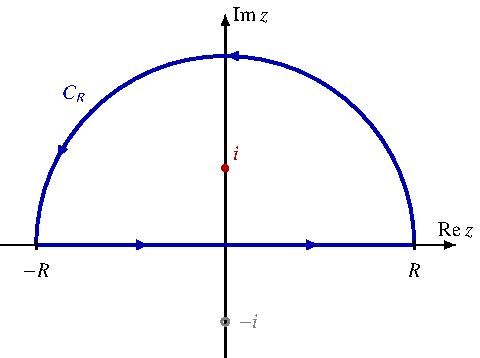
\includegraphics{papers/hauptwert/images/halbkreis-ohne-pol.pdf}
\caption{Halbkreiskontur ohne Polstelle auf der reellen Achse.
Der geschlossene Weg besteht aus der Strecke $[-R,R]$ und dem grossen
Halbkreis $C_R$ und wird im positiven Sinn durchlaufen.
Von den beiden Polstellen von $1/(1+z^2)$ liegt einzig $i$ im umlaufenen
Gebiet, während $-i$ in der unteren Halbebene keinen Beitrag liefert.
\label{hauptwert:figure:halbkreis-ohne-pol}}
\end{figure}
